\begin{center}
    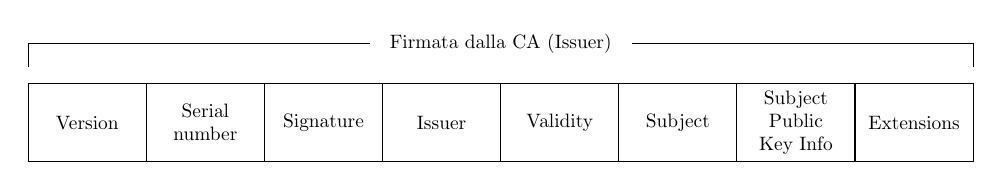
\begin{tikzpicture}
        \draw (0,0) -- ++(12,0);
        \draw (0,1) -- ++(12,0);

        \foreach \x in {0,1.5,...,12}
            \draw (\x,0) -- ++(0,1);

        \node[scale=0.7,align=center,text width=1.7cm] at (0.75,.5) {Version};
        \node[scale=0.7,align=center,text width=1.7cm] at (2.25,.5) {Serial number};
        \node[scale=0.7,align=center,text width=1.7cm] at (3.75,.5) {Signature};
        \node[scale=0.7,align=center,text width=1.7cm] at (5.25,.5) {Issuer};
        \node[scale=0.7,align=center,text width=1.7cm] at (6.75,.5) {Validity};
        \node[scale=0.7,align=center,text width=1.7cm] at (8.25,.5) {Subject};
        \node[scale=0.7,align=center,text width=1.7cm] at (9.75,.5) {Subject Public Key Info};
        \node[scale=0.7,align=center,text width=1.7cm] at (11.25,.5) {Extensions};
        \node[scale=0.7,align=center,text width=4.5cm] (CA) at (6,1.5) {Firmata dalla CA (Issuer)};

        \draw (0,1.2) |- (CA);
        \draw (12,1.2) |- (CA);
        
    \end{tikzpicture}
\end{center}